\documentclass[10pt, landscape]{article}
\usepackage[scaled=0.92]{helvet}
\usepackage{calc}
\usepackage{multicol}
\usepackage{ifthen}
\usepackage[a4paper,margin=3mm,landscape]{geometry}
\usepackage{amsmath,amsthm,amsfonts,amssymb}
\usepackage{color,graphicx,overpic}
\usepackage{hyperref}
\usepackage{newtxtext} 
\usepackage{enumitem}
\usepackage[table]{xcolor}
\usepackage{mathtools}
\usepackage{nicematrix}
% for drawing diragrams/graphs
\usepackage{tikz}
\usetikzlibrary{arrows.meta}
\usetikzlibrary{calc}
\setlist{nosep}

% ADDITIONAL USEFUL PACKAGES:
% for matrices

% for relations
\usepackage{cancel}
\usepackage{ mathrsfs }
% for including images
\graphicspath{ {./images/} }


\pdfinfo{
  /Title (MA1101R.pdf)
  /Creator (TeX)
  /Producer (pdfTeX 1.40.0)
  /Author (Jovyn)
  /Subject (MA1101R)
  /Keywords (MA1101R, nus,cheatsheet,pdf)}

% Turn off header and footer
\pagestyle{empty}

\newenvironment{tightcenter}{%
  \setlength\topsep{0pt}
  \setlength\parskip{0pt}
  \begin{center}
}{%
  \end{center}
}

% redefine section commands to use less space
\makeatletter
\renewcommand{\section}{\@startsection{section}{1}{0mm}%
                                {-1ex plus -.5ex minus -.2ex}%
                                {0.5ex plus .2ex}%x
                                {\normalfont\large\bfseries}}
\renewcommand{\subsection}{\@startsection{subsection}{2}{0mm}%
                                {-1explus -.5ex minus -.2ex}%
                                {0.5ex plus .2ex}%
                                {\normalfont\normalsize\bfseries}}
\renewcommand{\subsubsection}{\@startsection{subsubsection}{3}{0mm}%
                                {-1ex plus -.5ex minus -.2ex}%
                                {1ex plus .2ex}%
                                {\normalfont\small\bfseries}}%
\renewcommand{\familydefault}{\sfdefault}
\renewcommand\rmdefault{\sfdefault}
%  makes nested numbering (e.g. 1.1.1, 1.1.2, etc)
\renewcommand{\labelenumii}{\theenumii}
\renewcommand{\theenumii}{\theenumi.\arabic{enumii}.}
\renewcommand\labelitemii{•}
%  highlighting for math
\newcommand{\mathcolorbox}[2]{\colorbox{#1}{$\displaystyle #2$}}
%  convenient absolute value symbol
\newcommand{\abs}[1]{\vert #1 \vert}
%  convenient floor and ceiling
\newcommand{\floor}[1]{\lfloor #1 \rfloor}
\newcommand{\ceil}[1]{\lceil #1 \rceil}
%  convenient modulo
\newcommand{\Mod}[1]{\ \mathrm{mod}\ #1}
%  for logical not operator, iff symbol, convenient "if/then"
\renewcommand{\lnot}{\mathord{\sim}}
\let\iff\leftrightarrow
\let\Iff\Leftrightarrow
\let\then\rightarrow
\let\Then\Rightarrow
%  vectors
\newcommand{\vv}[1]{\boldsymbol{#1}}
\newcommand{\VV}[1]{\overrightarrow{#1}}
%  column vector
\newcommand{\cvv}[1]{\left(\begin{smallmatrix}#1\end{smallmatrix}\right)}
%  cell colours
\newcommand\bggreen{\cellcolor{green!10}}

\makeatother
\definecolor{myblue}{cmyk}{1,.72,0,.38}
\everymath\expandafter{\the\everymath \color{myblue}}
% Define BibTeX command
\def\BibTeX{{\rm B\kern-.05em{\sc i\kern-.025em b}\kern-.08em
    T\kern-.1667em\lower.7ex\hbox{E}\kern-.125emX}}

% Don't print section numbers
\setcounter{secnumdepth}{0}

\setlength{\parindent}{0pt}
\setlength{\parskip}{0pt plus 0.5ex}
%% this changes all items (enumerate and itemize)
\setlength{\leftmargini}{0.5cm}
\setlength{\leftmarginii}{0.5cm}
\setlist[itemize,1]{leftmargin=2mm,labelindent=1mm,labelsep=1mm}
\setlist[itemize,2]{leftmargin=4mm,labelindent=1mm,labelsep=1mm}

%My Environments
\newtheorem{example}[section]{Example}
% -----------------------------------------------------------------------

\begin{document}
\raggedright
\footnotesize
\begin{multicols*}{4
    '}


% multicol parameters
% These lengths are set only within the two main columns
\setlength{\columnseprule}{0.25pt}
\setlength{\premulticols}{1pt}
\setlength{\postmulticols}{1pt}
\setlength{\multicolsep}{1pt}
\setlength{\columnsep}{2pt}

\begin{center}
    \fbox{%
        \parbox{0.8\linewidth}{\centering \textcolor{black}{
            {\Large\textbf{MA1101R}}
            \\ \normalsize{AY20/21 sem 2}}
            \\ {\footnotesize \textcolor{myblue}{by jovyntls}}
        }%
    }
\end{center}

\section{01. LINEAR SYSTEMS}
\begin{itemize}
  \item \textbf{zero equation} $\then$ coefficients are all zero 
  \begin{itemize}
    \item either 0 or infinitely many solutions
  \end{itemize}
  \item \textbf{inconsistent} $\then$ has no solutions
  \item \textbf{solution set} $\then$ \textit{set} of all solutions to the equation
  \begin{itemize}
    \item $\{(1+s, 2s, s) \mid s \in \mathbb{R} \}$
  \end{itemize}
  \item \textbf{general solution} $\then$ \textit{expression} that gives us all solutions to the equation
  \begin{itemize}
    \item $\begin{cases}
      x=t
      \\ y = 2t + 1
    \end{cases}$
  \end{itemize}
\end{itemize}
\begin{center}
  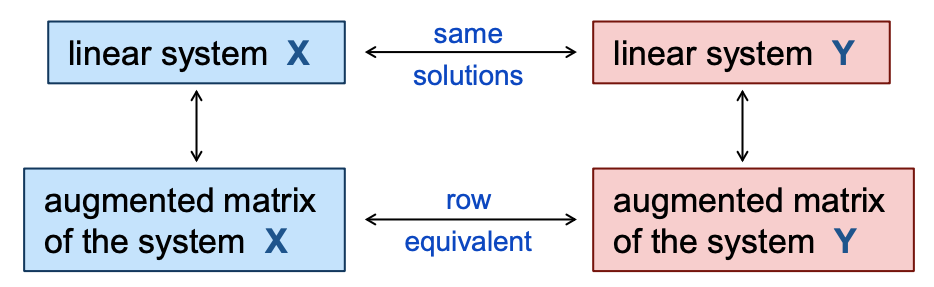
\includegraphics[width=0.9\linewidth]{ma1101r-ch1-1.png}
\end{center}

\subsection{elementary row operations}
\begin{enumerate}
  \item $cR_i, c\neq 0$ - multiply by a non-zero constant 
  \item $R_i \leftrightarrow R_j$ - interchange 2 equations
  \item $R_i + cR_j, c \in \mathbb{R}$ - add a multiple of one equation to another equation
\end{enumerate}

\subsection{(reduced) row echelon forms}
\begin{itemize}
  \item \# of pivot columns = \# of leading entries = \# of nonzero rows
  \item every matrix has a \textbf{unique} RREF but can have multiple REF.
\end{itemize}

\subsection{homogenous linear systems}
\begin{itemize}
  \item \textbf{homogenous} $\then$ rightmost column is all zeros 
  \item either:
  \begin{itemize}
    \item one solution - \textbf{trivial solution}
    \item infinitely many solutions AND the trivial solution
  \end{itemize}
\end{itemize}

\section{02. MATRICES}
\subsection{types of matrices}
\begin{itemize}
  \item \textbf{row/column} matrix $\then$ only one row/column
  \begin{itemize}
    \item 1x1 matrix is both row \& column matrix
  \end{itemize}
  \item \textbf{square} $\then$ same number of rows \& columns
  \item \textbf{diagonal} $\then$ all non-diagonal entries are zero
  \begin{itemize}
    \item \textbf{scalar} $\then$ all diagonal entries are the same
    \item \textbf{identity}, $I_n \then$ all diagonal entries are 1
  \end{itemize}
  \item \textbf{zero} $\then$ all entries are equal to zero
  \item \textbf{symmetric} $\then$ $a_{ij} = a_{ji} \forall i, j$
  \begin{itemize}
    \item symmetric $\iff A^T = A$
  \end{itemize}
  \item \textbf{triangular} 
  \begin{itemize}
    \item \textbf{upper} $\then a_{ij} = 0$ whenever $i>j$
    \item \textbf{lower} $\then a_{ij} = 0$ whenever $i<j$
    \item for any upper triangular matrix $D$ where all entries are 1, $D^n=0$.
  \end{itemize}
\end{itemize}

\subsection{useful notation}
<fill in lol>

\subsection{transpose}
\begin{itemize}
  \item $(A^T)^T = A$
  \item $(A+B)^T = A^T + B^T$
  \item if $c$ is a scalar, then $(cA)^T = cA^T$
  \item $(AB)^T = B^TA^T$
\end{itemize}

\subsection{inverse}
\begin{itemize}
  \item \textbf{uniqueness of inverses} $\then$ if $B$ and $C$ are inverses of $A$, then $B=C$.
  \item \textbf{cancellation laws} - only hold if $A$ is invertible.
  \begin{itemize}
    \item if $B_1$ and $B_2$ are $m \times n$ matrices such that $AB_1 = AB_2$, then $B_1 = B_2$.
    \item if $C_1$ and $C_2$ are $m \times n$ matrices such that $C_1A = C_2A$, then $C_1 = C_2$.
  \end{itemize}
\end{itemize}
\begin{center}
  inverse of 2x2 matrix:
  \\* $A^{-1} = \frac{1}{ad-bc} \left[ 
    \begin{array}{cc}
    d & -b\\
    -c & a
    \end{array}
    \right]$
\end{center}

\subsubsection{properties of inverses}
if $A, B$ are invertible matrices and $c$ is a nonzero scalar,
\begin{itemize}
  \item $cA$ is invertible: $(cA)^{-1} = \frac{1}{c}A^{-1}$
  \item $A^T$ is invertible: $(A^T)^{-1} = (A^{-1})^T$
  \item $A^{-1}$ is invertible: $(A^{-1})^{-1} = A$
  \item $AB$ is invertible: $(AB)^{-1} = B^{-1}A^{-1}$
\end{itemize}
\ 
\\ if $A,B$ are square matrices of the same size and $AB=I$, then
\begin{itemize}
  \item $A$ and $B$ are invertible
  \item $A^{-1} = B; \quad B^{-1}=A$
  \item $BA=I$
\end{itemize}
\ 
\\ negative powers of square matrices
\begin{itemize}
  \item $A^{-n} = (A^{-1})^n = A^{-1}A^{-1} \cdots A^{-1}$
  \item if $A$ is invertible, $(A^n)^{-1} = (A^{-1})^n$
\end{itemize}

% \begin{equation*}
%   \left[
%     \begin{array}{ccc}
%       x & x & x \\
%       0 & x & x \\
%       \rowcolor{blue!20}
%       0 & 0 & x \\
%       0 & 0 & 0 \\
%       \bggreen a  & \bggreen c &  d\\
%     \end{array}
%   \right]
% \end{equation*}




\end{multicols*}

\end{document}